\section{Aufbau und Durchführung}
\subsection{Aufbau}
Wie in Kapitel \ref{sec:1} beschrieben, wird die Lebensdauer der einzelnen Myonen bestimmt, indem die Zeitdifferenz zwischen Eintreffen
des Myons im Szintillator und dem folgenden Zerfall gemessen wird. Zur Zeitmessung werden die Signale des Szintillators als
Start- und Stopp-Impulse an einen Zeit-Amplituden-Konverter übertragen. Dabei kann nicht zwischen Myonen-Signalen und Zerfalls-Signalen
unterschieden werden. Problematisch hierbei ist, dass die meisten Myonen eine so hohe Energie haben, dass
sie im Szintillator nicht vollständig abgebremst werden und somit nicht innerhalb des Szintillators zerfallen.
Diese Myonen senden also nur ein Start-Signal bei ihrem Eintreffen, aber kein Stopp-Signal, da sie nicht im Szintillator zerfallen,
sodass solche Signale abgefangen werden müssen. Weiterhin zerfallen nicht alle negativen Myonen sofort,
sondern manche werden zunächst von einem Atomkern eingefangen und bilden ein myonisches Atom.

\begin{figure}[h]
  \centering
  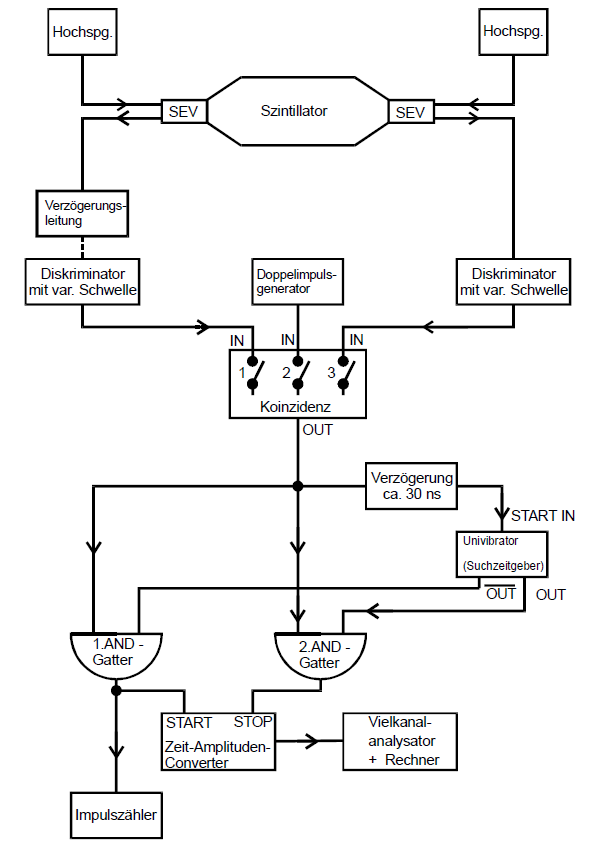
\includegraphics[scale=1.2]{graphics/aufbau.png}
  \caption{Schematischer Versuchsaufbau, nach \cite{anleitung}.}
  \label{fig:aufbau}
\end{figure}

In Abbildung \ref{fig:aufbau} ist der verwendete Versuchsaufbau schematisch dargestellt. Aufgrund der benötigten geringen Abklingzeit wird ein organischer Szintillator
verwendet. Dieser hat gegenüber anorganischen Szintillatoren den Nachteil, dass keine gute Energieauflösung erreicht wird, allerdings wird hier keine Messung der
Energie benötigt, sodass dieser Nachteil für die Durchführung irrelevant ist.
Wie in der Abbildung deutlich wird, werden an zwei entgegengesetzten Seiten Sekundärelektronenverstärker (SEV) optisch angekoppelt. Diese wandeln die Lichtimpulse
des Szintillators in elektronische Impulse um. Ein Problem bei den SEV besteht darin, dass sie zu spontaner Elektronenemission neigen, welche die Messungen
verfälschen können. Deshalb werden zwei SEV verwendet und eine Koinzidenzschaltung verwendet, die nur Signale zulässt, wenn die beiden SEV innerhalb eines kurzen Intervalls \enquote{gleichzeitig}
Impulse liefern. Da die beiden SEV und deren optische Kopplung an den Szintillator leichte Unterschiede aufweisen können, wird beiden SEV jeweils eine Verzögerungsleitung nachgeschaltet, die
so angepasst wird, dass die Signale zeitgleich bei der Koinzidenzschaltung ankommen. Vor der Koinzidenzschaltung ist jeweils ein Diskriminator, der zum einen der Rauschunterdrückung dient,
indem er sämtliche Signale unterhalb einer einstellbaren Schwelle herausfiltert,
und zum anderen die Signale der SEV auf eine einheitliche Länge und Breite bringt, da die restliche Schaltung aus logischen Bauteilen besteht, welche dem NIM-Standard folgen.

Da die mittlere Lebensdauer der Myonen kleiner als der mittlere zeitliche Abstand zwischen zwei einfallenden Myonen ist, kann die Lebensdauer mithilfe einer Stoppuhr gemessen werden.
Die Stoppuhr wird durch den Impuls eines einfallenden Myons gestartet und durch den Impuls des zerfallenden Myons gestoppt. Dazu wird ein Zeit-Amplituden-Converter (TAC) verwendet,
der einen Spannungsimpuls abgibt, dessen Amplitude proportional
zur Zeitdifferenz zwischen Start- und Stoppsignal ist. Außerdem werden die Start- und Stoppimpulse, die den TAC erreichen, von Impulszählern aufgezeichnet. Die Impulse des TAC werden von einem
Vielkanalanalysator entsprechend ihrer Höhe in 512 Kanälen histogrammiert. Zur Kalibrierung der Kanäle kann an die Koinzidenzschaltung ein Doppelimpulsgenerator angeschlossen werden, welcher
elektrische Impulse mit einer einstellbaren Zeitdifferenz erzeugen kann.

Zu berücksichtigen ist jedoch, dass die meisten Myonen zu hochenergetisch sind, sodass sie durch den Szintillator durchgehen und nicht darin komplett abgebremst werden. Dadurch geben diese
nur einen Startimpuls und keinen Stoppimpuls. Es wird also eine logische Schaltung mithilfe eines Univibrators und zweier AND-Gatter aufgebaut, die die Schaltung nach einer einstellbaren
Suchzeit $T_\text{S}$ wieder in ihren Ausgangszustand versetzt, sodass nach Ablauf dieser Zeit das nächste Signal wieder als Startsignal gewertet wird. Da die Signale der Koinzidenzschaltung
eine Länge von ca. $\SI{20}{ns}$ haben, ist vor dem Univibrator eine Verzögerungsleitung mit einer Verzögerung von ca. $\SI{30}{ns}$ eingebaut.
Zu Beginn der Messung liegt am Ausgang des Univibrators ein L-Signal an, am invertierten Ausgang also ein H-Signal, sodass ein Signal von der Koinzidenzschaltung das 1. AND-Gatter passieren kann
und die Zeitmessung am TAC startet. Nach der Verzögerung von $\SI{30}{ns}$ erreicht das Signal der Koinzidenzschaltung den Univibrator, welcher die Suchzeit startet. Während der Suchzeit liegt
am Ausgang des Univibrators ein H-Signal an sodass ein Signal von der Koinzidenzschaltung nur das 2. AND-Gatter passiert und nicht das 1., sodass ein Stopp-Signal am TAC ankommt. Nach Ablauf der
Suchzeit oder nach Eintreffen eines Signals springt der Univibrator zurück in seinen Ausgangszustand, sodass das nächste Signal wieder nur das 1. AND-Gatter passieren kann, die Zeitmessung des TACs
also neu startet.

Trotz des Herausfilterns vieler Störeffekte bleibt ein Untergrund übrig, da es eine endliche Wahrscheinlichkeit gibt, dass innerhalb der Suchzeit zwei Myonen hintereinander eintreffen, sodass
die Zeitdifferenz zwischen den beiden Myonen als Lebensdauer aufgezeichnet wird, obwohl die Myonen nicht in dem Zeitraum zerfallen sind. Da eintreffende Myonen und zerfallende Myonen nicht voneinander
unterschieden werden können, kann dieser Untergrund bei der Versuchsdurchführung nicht herausgefiltert werden, sondern muss bei der Auswertung berücksichtigt werden.

\subsection{Durchführung}
Zunächst muss die Schaltung aufgebaut werden und die einzelnen Komponenten müssen eingestellt werden. Angefangen wird bei den Diskriminatorschwellen, die so eingestellt werden, dass
beide Diskriminatoren die gleiche Impulsrate liefern, welche zwischen 20 und 40 Impulsen pro Sekunde liefen sollte. Um keine Myonen-Signale zu verlieren, sollte die Impulsrate allerdings näher an 40
Impulsen pro Sekunde liegen. Dann werden die Verzögerungsleitungen so aufeinander eingestellt, dass
die maximale Anzahl an Impulsen von der Koinzidenzschaltung ausgegeben werden. Danach wird ein Oszilloskop an den Ausgang des Univibrators angeschlossen, um die Suchzeit $T_\text{S}$ einzustellen.
Gewählt wird eine Suchzeit von $\SI{20}{\micro\second}$. Nun wird die Schaltung bis zum TAC aufgebaut und dessen Funktionsweise überprüft. Dazu wird der Doppelimpulsgenerator anstelle der SEV an die
Koinzidenzschaltung angeschlossen. Der Messbereich des TACs wird an die Suchzeit $T_\text{S}$ angepasst. Zuletzt wird der Vielkanalanalysator angeschlossen und kalibriert. Dazu werden mit dem Doppelimpulsgenerator
Impulse mit verschiedenen Zeitdifferenzen erzeugt und überprüft, welche Kanäle diesen Zeitdifferenzen entsprechen. Daraus kann eine Ausgleichsgerade für den Zusammenhang zwischen Kanalnummer und Zeitdifferenz berechnet
werden.

Nach dem Aufbau der Schaltung und der Kalibrierung wird das Messprogramm gestartet und zeitgleich werden die Impulszähler gestartet. Über einen Zeitraum von $\SI{45.11}{\hour}$ werden Daten aufgenommen.
